\documentclass[a4paper, 12pt]{article}

\usepackage[english,russian]{babel}
\usepackage[T2A]{fontenc}
\usepackage[utf8]{inputenc}
\usepackage{geometry}
\usepackage{enumitem}
\usepackage{setspace}
\usepackage{amssymb}
\usepackage{graphicx}
\usepackage{wrapfig}
\usepackage{float}
\usepackage{amsmath}
\usepackage{textcomp}
\usepackage{dsfont}

\geometry{top=5mm, left=1cm}
%\setlength{\parindent}{0}
\renewcommand{\arraystretch}{1.2}
\linespread{1}

\begin{document}
    \begin{center}
        \textbf{Сферическая геометрия №5}\\
        Теорема косинусов, теорема синусов.
    \end{center}

    \begin{center}
        \textbf{№ 1}
    \end{center}

    На сфере радиуса $R$ дан треугольник с сторонами $a, b, c$ найдите его площадь.

    \textbf{Решение}\\

    \begin{center}
        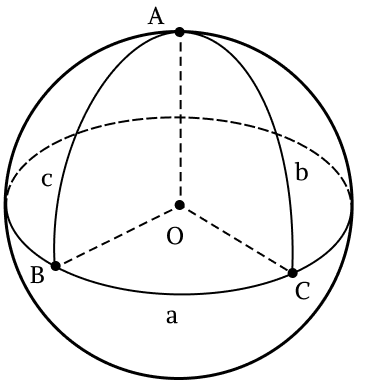
\includegraphics[width=0.2\textwidth]{images/img3}\\
    \end{center}

    1) По сферической теореме косинусов:
    \[
        \begin{cases}
            \cos \frac{a}{R} = \cos \frac{b}{R}\cos\frac{c}{R} + \sin \frac{b}{R}\sin\frac{c}{R}\cos A\\
            \cos \frac{b}{R} = \cos \frac{a}{R}\cos\frac{c}{R} + \sin \frac{a}{R}\sin\frac{c}{R}\cos B\\
            \cos \frac{c}{R} = \cos \frac{a}{R}\cos\frac{b}{R} + \sin \frac{a}{R}\sin\frac{b}{R}\cos C\\
        \end{cases}
        \rightarrow
    \]
    \[
        \begin{cases}
            \cos A = \frac{\cos \frac{a}{R} - \cos \frac{b}{R}\cos\frac{c}{R}}{\sin \frac{b}{R}\sin\frac{c}{R}}\\
            \cos B = \frac{\cos \frac{b}{R} - \cos \frac{a}{R}\cos\frac{c}{R}}{\sin \frac{a}{R}\sin\frac{c}{R}}\\
            \cos C = \frac{\cos \frac{c}{R} - \cos \frac{a}{R}\cos\frac{b}{R}}{\sin \frac{a}{R}\sin\frac{b}{R}}\\
        \end{cases}
    \]

    2) Следовательно площадь равна:
    \[
        S = R^2\left(\arccos \frac{\cos \frac{a}{R} - \cos \frac{b}{R}\cos\frac{c}{R}}{\sin \frac{b}{R}\sin\frac{c}{R}} -
        + \arccos  \frac{\cos \frac{b}{R} - \cos \frac{a}{R}\cos\frac{c}{R}}{\sin \frac{a}{R}\sin\frac{c}{R}}
        + \arccos \frac{\cos \frac{c}{R} - \cos \frac{a}{R}\cos\frac{b}{R}}{\sin \frac{a}{R}\sin\frac{b}{R}}\\
        \pi\right)
    \]

    \begin{center}
        \textbf{№ 2}
    \end{center}

    На сфере радиуса $R$ дан треугольник со сторонами $a, b, c$.
    Угол между $a$ и $b$ равен $C$.
    Найдите чему равна сторона $c$, если радиус сферы $R$.

    \textbf{Решение}\\

    \begin{center}
        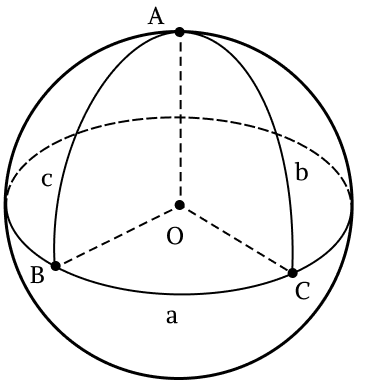
\includegraphics[width=0.2\textwidth]{images/img4}\\
    \end{center}

    1) По сферической теореме косинусов:
    \[
        \cos \frac{c}{R} = \cos\frac{a}{R}\cos\frac{b}{R} + \sin\frac{a}{R}\sin\frac{b}{R}\cos C
    \]
    \[
        \frac{c}{R} = \arccos\left( \cos\frac{a}{R}\cos\frac{b}{R} + \sin\frac{a}{R}\sin\frac{b}{R}\cos C\right)
    \]
    \[
        c = R\arccos\left( \cos\frac{a}{R}\cos\frac{b}{R} + \sin\frac{a}{R}\sin\frac{b}{R}\cos C\right)
    \]

    \begin{center}
        \textbf{№ 3}
    \end{center}

    Через боковые стороны равнобедренного сферического треугольника провели среднюю линию.
    Найдите длину средней линии, если известны стороны исходного треугольника и угол противолежащий основанию.

    \textbf{Решение}\\

    \begin{center}
        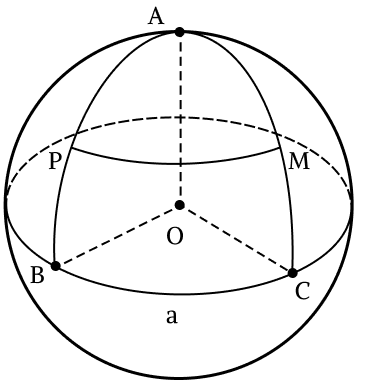
\includegraphics[width=0.2\textwidth]{images/img5}\\
    \end{center}

    1) По теореме косинусов в $\triangle PAM$
    \[
        \cos \frac{PM}{R} = \cos \frac{AP}{R}\cos\frac{AM}{R} + \sin\frac{AP}{R}\sin\frac{AM}{R}\cos A
    \]
    \[
        PM = R\arccos \left(\cos \frac{AP}{R}\cos\frac{AM}{R} + \sin\frac{AP}{R}\sin\frac{AM}{R}\cos A\right) =
    \]
    \[
        R\arccos \left(\cos \frac{AB}{2R}\cos\frac{AC}{2R} + \sin\frac{AB}{2R}\sin\frac{AC}{2R}\cos A\right) =
    \]

    \begin{center}
        \textbf{№ 4}
    \end{center}

    Через боковые стороны равнобедренного сферического треугольника провели среднюю линию.
    Найдите углы получившегося треугольника, если известны стороны исходного треугольника и угол противолежащий основанию.

    \textbf{Решение}\\

    \begin{center}
        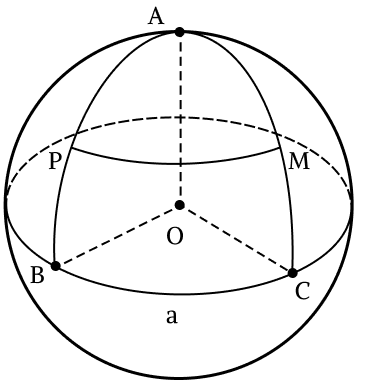
\includegraphics[width=0.2\textwidth]{images/img6}\\
    \end{center}

    1) Рассмотрим $\triangle APM$:
    \[
        \begin{cases}
            \cos \frac{AP}{R} = \cos \frac{PM}{R}\cos\frac{AM}{R} + \sin \frac{PM}{R}\sin\frac{AM}{R}\cos M\\
            \cos \frac{AM}{R} = \cos \frac{AP}{R}\cos\frac{PM}{R} + \sin \frac{AP}{R}\sin\frac{PM}{R}\cos P\\
            \cos \frac{PM}{R} = \cos \frac{AP}{R}\cos\frac{AM}{R} + \sin \frac{AP}{R}\sin\frac{AM}{R}\cos A\\
        \end{cases}
        \rightarrow
    \]
    \[
        \begin{cases}
            M = \arccos \frac{\cos \frac{AP}{R} - \cos \frac{PM}{R}\cos\frac{AM}{R}}{\sin \frac{PM}{R}\sin\frac{AM}{R}}=
            \arccos \frac{\cos \frac{AB}{2R} - \cos \frac{PM}{R}\cos\frac{AC}{2R}}{\sin \frac{PM}{R}\sin\frac{AC}{2R}}\\
            P = \arccos \frac{\cos \frac{AM}{R} -  \cos \frac{AP}{R}\cos\frac{PM}{R}}{\sin \frac{AP}{R}\sin\frac{PM}{R}}=
            \arccos \frac{\cos \frac{AC}{2R} -  \cos \frac{AB}{2R}\cos\frac{PM}{R}}{\sin \frac{AB}{2R}\sin\frac{PM}{R}}\\
            A = \arccos \frac{\cos \frac{PM}{R} - \cos \frac{AP}{R}\cos\frac{AM}{R}}{\sin \frac{AP}{R}\sin\frac{AM}{R}}=
            \arccos \frac{\cos \frac{PM}{R} - \cos \frac{AB}{2R}\cos\frac{AC}{2R}}{\sin \frac{AB}{2R}\sin\frac{AC}{2R}}\\
        \end{cases}
    \]

    Средняя линия была найдена в предыдущей задаче.

    \begin{center}
        \textbf{№ 5}
    \end{center}

    В сферическом треугольнике известны три стороны и один угол.
    Найдите остальные углы.

    \textbf{Решение}\\

    \begin{center}
        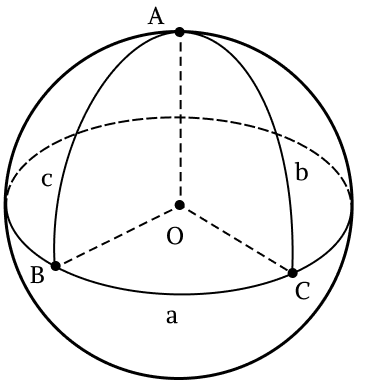
\includegraphics[width=0.2\textwidth]{images/img7}\\
    \end{center}

    1) По теореме синусов:
    \[
        \frac{\sin\frac{a}{R}}{\sin A} = \frac{\sin\frac{b}{R}}{\sin B} = \frac{\sin\frac{c}{R}}{\sin C}
    \]
    Пусть известен угол $A$, тогда:
    \[
        B = \frac{\sin \frac{b}{R}\sin A}{\sin\frac{a}{R}}
    \]
    \[
        C = \frac{\sin\frac{c}{R}\sin A}{\sin\frac{a}{R}}
    \]

    \begin{center}
        \textbf{№ 6}
    \end{center}

    В сферическом треугольнике $ABC$ угол $B$ прямой.
    Найдите косинусы, синусы, тангенсы, котангенсы двух других углов,
    если известны стороны треугольника и радиус сферы.

    \textbf{Решение}\\

    \begin{center}
        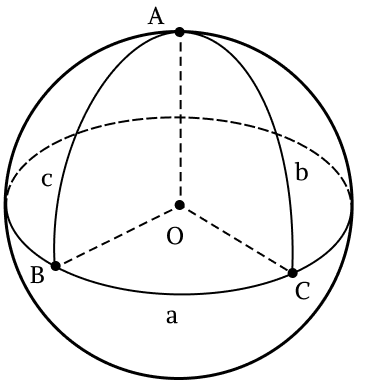
\includegraphics[width=0.2\textwidth]{images/img8}\\
    \end{center}

    1) По теореме синусов:
    \[
        \frac{\sin\frac{a}{R}}{\sin A} = \frac{\sin\frac{b}{R}}{\sin B} = \frac{\sin\frac{c}{R}}{\sin C}
    \]
    \[
        \sin A = \frac{\sin\frac{a}{R}}{\sin\frac{b}{R}}
    \]
    \[
        \sin C = \frac{\sin\frac{c}{R}}{\sin\frac{b}{R}}
    \]

    2) По теореме косинусов:
    \[
        \begin{cases}
            \cos\frac{a}{R} = \cos\frac{b}{R}\cos\frac{c}{R} + \sin\frac{b}{R}\sin\frac{c}{R}\cos A\\
            \cos\frac{c}{R} = \cos\frac{a}{R}\cos\frac{b}{R} + \sin\frac{a}{R}\sin\frac{b}{R}\cos C\\
        \end{cases}
        \rightarrow
    \]
    \[
        \begin{cases}
            \cos A = \frac{\cos\frac{a}{R} - \cos\frac{b}{R}\cos\frac{c}{R}}{\sin\frac{b}{R}\sin\frac{c}{R}}\\
            \cos C = \frac{\cos\frac{c}{R} - \cos\frac{a}{R}\cos\frac{b}{R}}{\sin\frac{a}{R}\sin\frac{b}{R}}\\
        \end{cases}
    \]

     \begin{center}
        \textbf{№ 7}
    \end{center}

    В сферическом треугольнике $ABC$ угол $B$ прямой.
    Найдите сторону $AC$, если известны все углы, сторона $AB$ и радиус сферы.

    \textbf{Решение}\\

    \begin{center}
        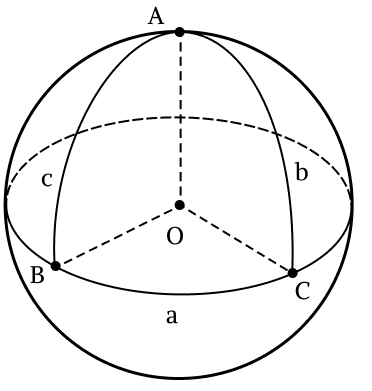
\includegraphics[width=0.2\textwidth]{images/img9}\\
    \end{center}

    1) По теореме синусов:
    \[
        \frac{\sin\frac{a}{R}}{\sin A} = \frac{\sin\frac{b}{R}}{\sin B} = \frac{\sin\frac{c}{R}}{\sin C}
    \]
    \[
        \sin\frac{b}{R} = \frac{\sin\frac{c}{R}}{\sin C}
    \]
    \[
        b = R\arcsin\left(\frac{\sin\frac{c}{R}}{\sin C}\right)
    \]

\end{document}
